% ─────────────────────────────────────────────────────────────
% ECE 370/590 — Laboratory Exercise 1: The Dipole Antenna
% Place this file in the "Lab 1" folder (next to Plots/ and Data/).
% Compile: latexmk -pdf lab1.tex
% ─────────────────────────────────────────────────────────────
\documentclass[11pt]{article}

\usepackage[margin=1in]{geometry}
\usepackage{amsmath,amssymb}
\usepackage{siunitx}
\usepackage{graphicx}
\usepackage{booktabs}
\usepackage{float}
\usepackage{caption}
\usepackage{subcaption}
\usepackage{xcolor}
\usepackage{enumitem}
\usepackage[framemethod=TikZ]{mdframed}
\usepackage{hyperref}
\usepackage{cleveref}

\sisetup{detect-all, per-mode=symbol}
\hypersetup{colorlinks=true, linkcolor=blue!50!black, citecolor=blue!50!black, urlcolor=blue!50!black}

% ── Paths ────────────────────────────────────────────────────
\newcommand{\simdir}{Plots/1 Inch}   % CST results, 1-in-wide copper tape
\newcommand{\measdir}{Data}          % LibreVNA exports and screenshots

% ── Helpers ──────────────────────────────────────────────────
\newcounter{labq}
\newmdenv[
  backgroundcolor=gray!10, linewidth=0pt,
  leftline=true, linecolor=gray!60, innerlinewidth=2pt,
  innertopmargin=6pt, innerbottommargin=6pt, skipabove=8pt, skipbelow=4pt
]{qbox}
\newenvironment{question}{\refstepcounter{labq}\begin{qbox}\textbf{Question \thelabq.}~}{\end{qbox}}
\newcommand{\answer}[1]{\par\noindent\textbf{Answer.}~#1\par\medskip}
\newcommand{\todo}[1][Answer here.]{\textcolor{red!60!black}{\textit{[#1]}}}

\title{ECE 370/590 Laboratory Exercise 1:\\ The Dipole Antenna}
\author{Roshan Sundaram, Samuel Rivera, Shreyas Banaji}
\date{\today}

\begin{document}
\maketitle

% ═════════════════════════════════════════════════════════════
\section{Analytical Design (Exercise 1.1)}

At $f = \SI{1}{GHz}$,
\begin{equation}
  \lambda = \frac{c}{f} = \frac{\SI{2.998e8}{m/s}}{\SI{1e9}{Hz}} = \SI{299.8}{mm},
  \qquad \frac{\lambda}{2} = \SI{149.9}{mm}.
\end{equation}

\begin{table}[H]
  \centering
  \caption{Initial design parameters.}
  \label{tab:design}
  \begin{tabular}{@{}lllp{0.3\linewidth}@{}}
    \toprule
    Parameter & Symbol & Value  \\
    \midrule
    Total length (tip to tip) & $L$ & \SI{150}{mm} \\
    Conductor & --- & Copper tape on foam board  \\
    Strip width & $w$ & \SI{25.4}{mm}   \\
    Tape thickness & $t$ & \SI{0.05}{mm}  \\
    Feed gap & $g$ & \SI{12.7}{mm}  \\
    \bottomrule
  \end{tabular}
\end{table}

\begin{question}What initial dimensions would you select for a dipole resonant near 1 GHz and why?\end{question}
\answer{Given that the wavelength of a 1 GHz signal is \SI{299.8}{mm}, a half-wave dipole would ideally have a length of \SI{149.9}{mm}. The CST simulation we used had a feed gap of \SI{0.5}{in} and assumed a strip width of \SI{1}{in}, so we built the antenna to be as representative of the simulated model as possible.}

\begin{question}What input resistance do you expect at resonance, and how does this compare with the 50~$\Omega$ impedance of the VNA?\end{question}
\answer{At resonance, we expect the input impedance of a half-wave dipole to be about $73 \Omega$. Since the VNA has an impedance of 50~$\Omega$, we expect a slight mismatch at the interface. }

\begin{question}How should the antenna impedance change as the length is increased or decreased?\end{question}
\answer{As we make the antenna longer, we expect the resonant frequency to decrease, meaning that we expect an impedance of 73~$\Omega$ at a lower frequency. Therefore, the input impedance at 1 GHz should increase as we increase the length of the antenna.}

\begin{question}How might the conductor diameter or width affect resonance and bandwidth?\end{question}
\answer{The conductor diameter affects the fractional bandwidth, $B$, according to:}
\begin{equation}
    B = \frac{\Delta f}{f_0} = \frac{4\sqrt{2}}{\pi^2} \cdot \frac{R_{\text{rad}}}{120 \left[ \ln\left(\frac{l}{d}\right) - 1 \right]}
\end{equation}
where $l$ is the length of the dipole and $d$ is the diameter. In the event that $d$ increases, $B$ would (generally) increase. As for the resonance frequency, we can assume that a larger diameter (or width) would cause the resonance frequency to decrease.

% ═════════════════════════════════════════════════════════════
\section{CST Simulation (Exercise 1.2)}

\subsection{Model setup}

We modeled the copper tape dipole matching our analytical design. Out of the available solvers, we chose to use the time domain solver between 0.5 - 1.5 GHz. The antenna's feed was modeled using a discrete port. The port was assigned an impedance of 50 ohms and the ``substrate'' was modeled using a vacuum. This is because we plan to fabricate the antenna using a thin poster board rather than a traditional substrate like FR-4.
% \todo[Solver (time domain), frequency range \SIrange{0.7}{1.3}{GHz}, open (add space) boundaries, discrete \SI{50}{\ohm} port across the feed gap, conductor material (copper vs.\ PEC), foam board included or not, mesh cell count and convergence check. State the simulated length $L$.]

\subsection{Reflection coefficient and input impedance}

\begin{figure}[H]
  \centering
  \includegraphics[width=\linewidth]{\simdir/S11.png}
  \caption{Simulated $|S_{11}|$ (dB) re \SI{50}{\ohm}, \SI{1}{in}-wide tape dipole. Minimum \SI{-15.1}{dB} near \SI{0.873}{GHz}; \SI{-8.14}{dB} at \SI{1}{GHz}.}
  \label{fig:sim-s11}
\end{figure}

\begin{figure}[H]
  \centering
  \includegraphics[width=\linewidth]{\simdir/S1,1_re_im.png}
  \caption{Simulated $S_{11}$, real and imaginary parts. At \SI{1}{GHz}: $S_{11} = 0.380 + j0.093$.}
  \label{fig:sim-s11-reim}
\end{figure}

\begin{figure}[H]
  \centering
  \includegraphics[width=\linewidth]{\simdir/Z1,1.png}
  \caption{Simulated input impedance $Z_{11}$. At \SI{1}{GHz}: $Z_{11} = 107.9 + j23.7~\Omega$. Reactance crosses zero near {0.90}{GHz}.}
  \label{fig:sim-z11}
\end{figure}

\begin{table}[H]
  \centering
  \caption{Simulated resonance summary (\SI{1}{in} tape, $L = $ 150mm.}
  \label{tab:sim-summary}
  \begin{tabular}{@{}lc@{}}
    \toprule
    Quantity & Value \\
    \midrule
    Zero-reactance frequency $f_{X=0}$ & \SI{0.904}{GHz} \\
    $R_\text{in}$ at $f_{X=0}$ & \SI{74.87}{\ohm} \\
    Frequency of min $|S_{11}|$ (Resonant Frequency) & \SI{0.873}{GHz} \\
    Min $|S_{11}|$ & \SI{-15.1}{dB} \\
    \SI{-10}{dB} band & \SIrange{0.807}{0.964}{GHz} \\
    Fractional bandwidth & $\approx$0.157 \\
    $Z_{11}$ at \SI{1}{GHz} & $107.9 + j23.7~\Omega$ \\
    Radiation efficiency at \SI{1}{GHz} & 0.9998 \\
    Directivity at \SI{1}{GHz} & \SI{2.19}{dBi} \\
    \bottomrule
  \end{tabular}
\end{table}

\subsection{Surface current and far field}

\begin{figure}[H]
  \centering
  \includegraphics[width=\linewidth]{\simdir/surface current (f=1) [1].png}
  \caption{Simulated surface current magnitude at \SI{1}{GHz} (max \SI{1.99}{A/m}).}
  \label{fig:sim-current}
\end{figure}

% NOTE: the curve evaluation below reads ~1e-8 A/m and is zero outside 68–82 mm,
% so the curve is probably not on the tape surface. Re-place it and re-evaluate
% before using this figure.
% \begin{figure}[H]
%   \centering
%   \includegraphics[width=\linewidth]{\simdir/curve1_h-field (f=1) (1).png}
%   \caption{Tangential $H$ (surface current density) along the dipole at \SI{1}{GHz}.}
%   \label{fig:sim-current-curve}
% \end{figure}

\begin{figure}[H]
  \centering
  \begin{subfigure}[b]{0.58\linewidth}
    \centering
    \includegraphics[width=\linewidth]{\simdir/farfield (f=1) [1].png}
    \caption{Directivity cut at \SI{1}{GHz} (main lobe \SI{2.19}{dBi}, \SI{3}{dB} width \SI{121.6}{\degree}).}
  \end{subfigure}\hfill
  \begin{subfigure}[b]{0.40\linewidth}
    \centering
    \includegraphics[width=\linewidth]{\simdir/Rad. Efficiency [1].png}
    \caption{Radiation efficiency at \SI{1}{GHz}: 0.9998.}
  \end{subfigure}
  \caption{Simulated far-field and efficiency.}
  \label{fig:sim-farfield}
\end{figure}

\subsection{Parameter sweep}
We selectively swept $L$ from \SI{150}{mm} to \SI{126}{mm} to see if we could shift the resonant frequency to $\approx$ 1 GHz. After the sweep, the best result was shown for $L = \SI{131}{mm}$. You will find that the 

\begin{figure}[H]
  \centering
  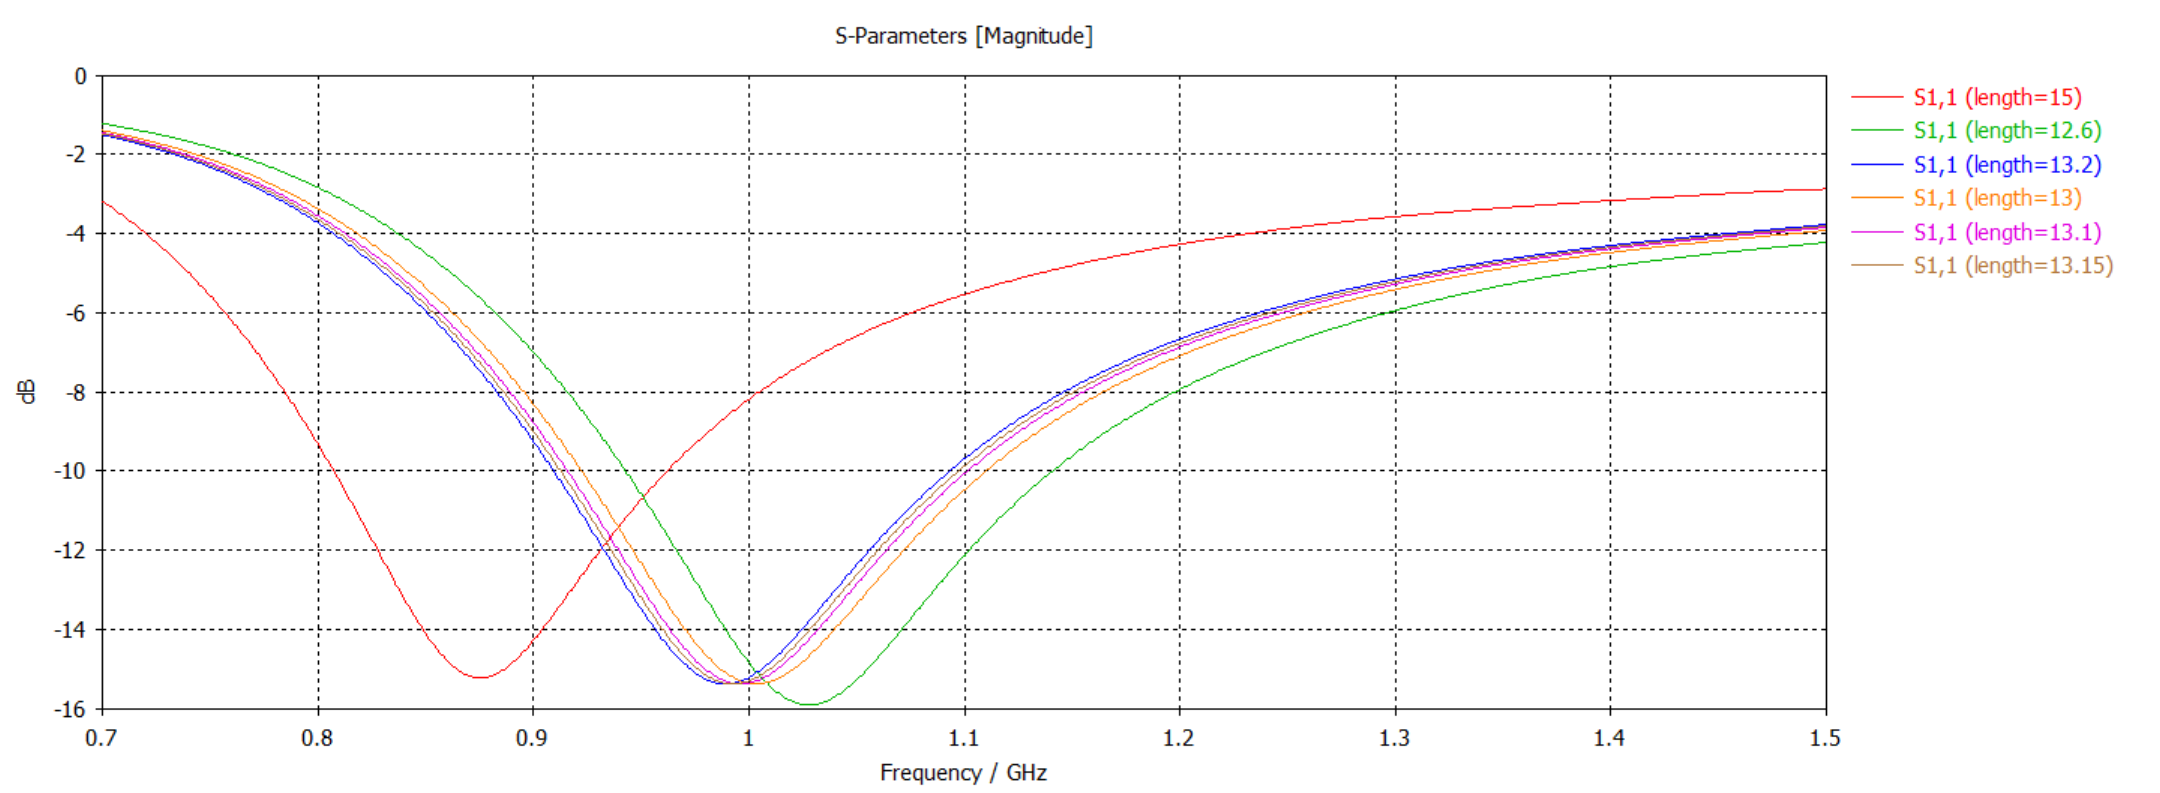
\includegraphics[width=0.8\linewidth]{Lab 1/Data/1_ghz_resonant.png}
  \caption{Simulated $|S_{11}|$ for $L = $ \SIrange{126}{150}{mm}.}
  \label{fig:sim-sweep}
\end{figure}

\begin{question}How closely does the simulated resonant length agree with your analytical estimate?\end{question}
\answer{The simulated resonant length, \SI{131}{mm}, is \SI{19}{mm} off of our analytical estimate. This is approximately $13\%$ decrease in length, so sizable to say the least.}
\begin{question}What happens to the input impedance as the dipole length changes?\end{question}
\answer{As the dipole length decreases, the input impedance also decreases.}
\begin{figure}[H]
    \centering
    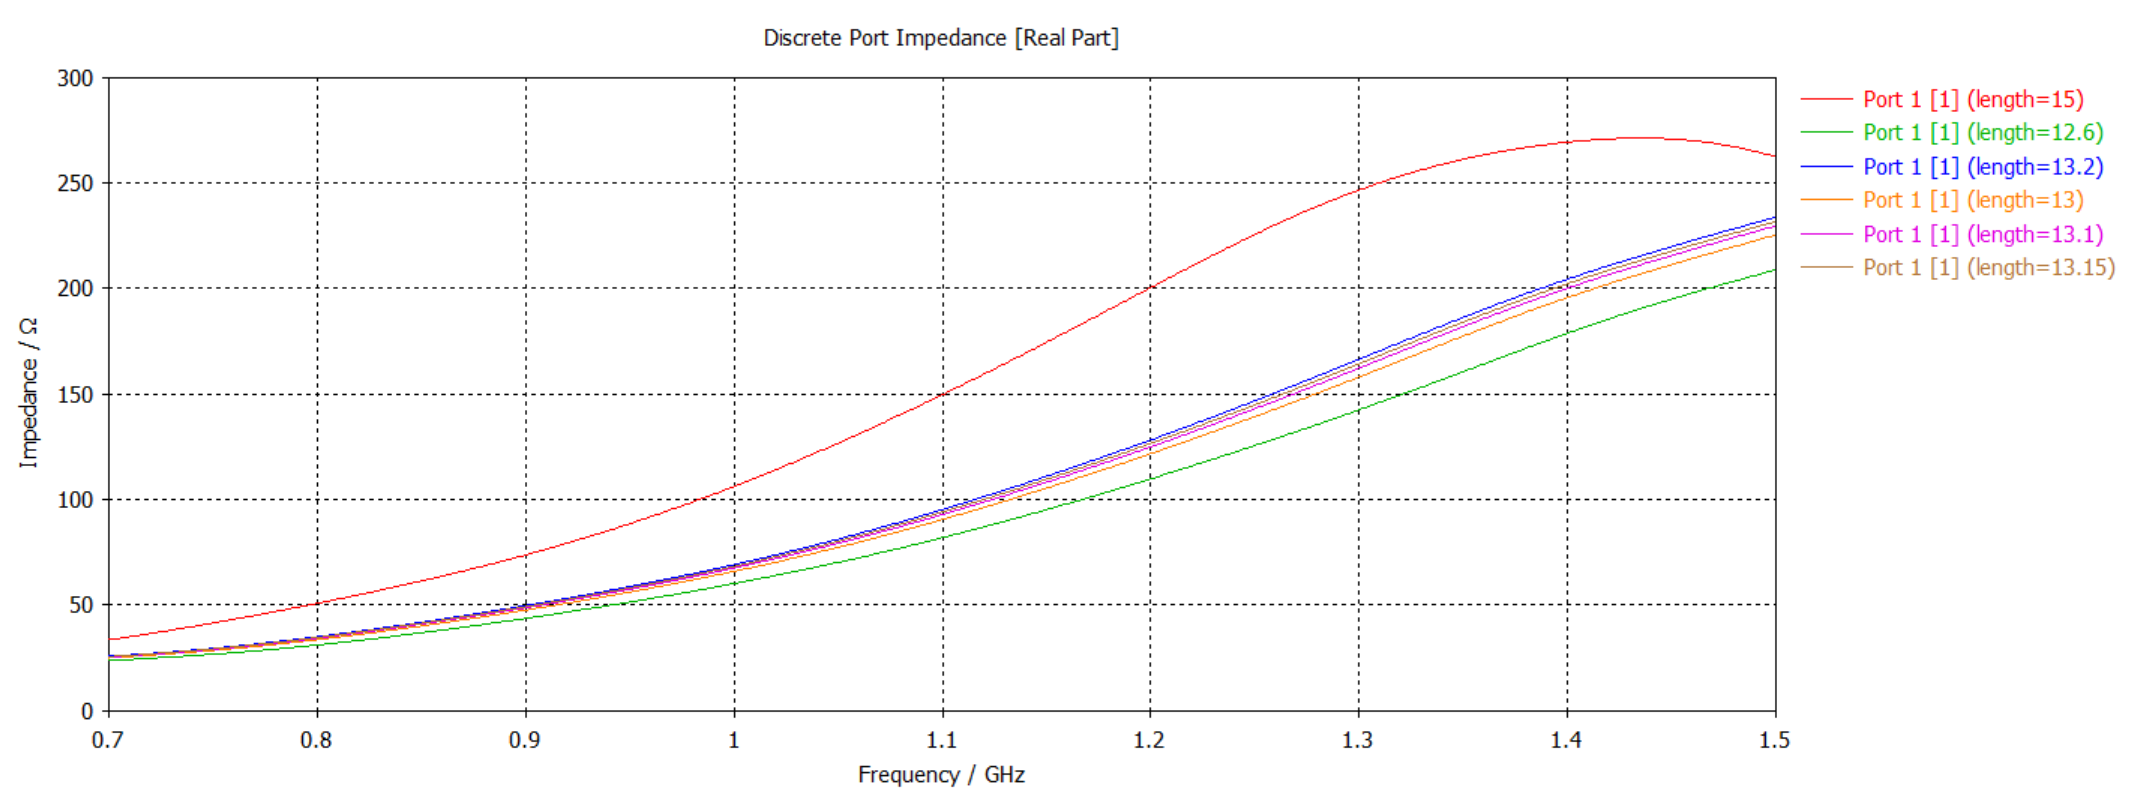
\includegraphics[width=0.8\linewidth]{Lab 1/Data/input_impedance.png}
    \caption{$L$ vs. Input Impedance (Real Part)}
    \label{fig:placeholder}
\end{figure}

\begin{question}How does the predicted bandwidth depend on conductor thickness or width?\end{question}
\answer{The predicted bandwidth shrinks as the conductor width decreases. We swept the simulation from \SI{254}{mm} to \SI{50}{mm}}.

\begin{figure}[H]
    \centering
    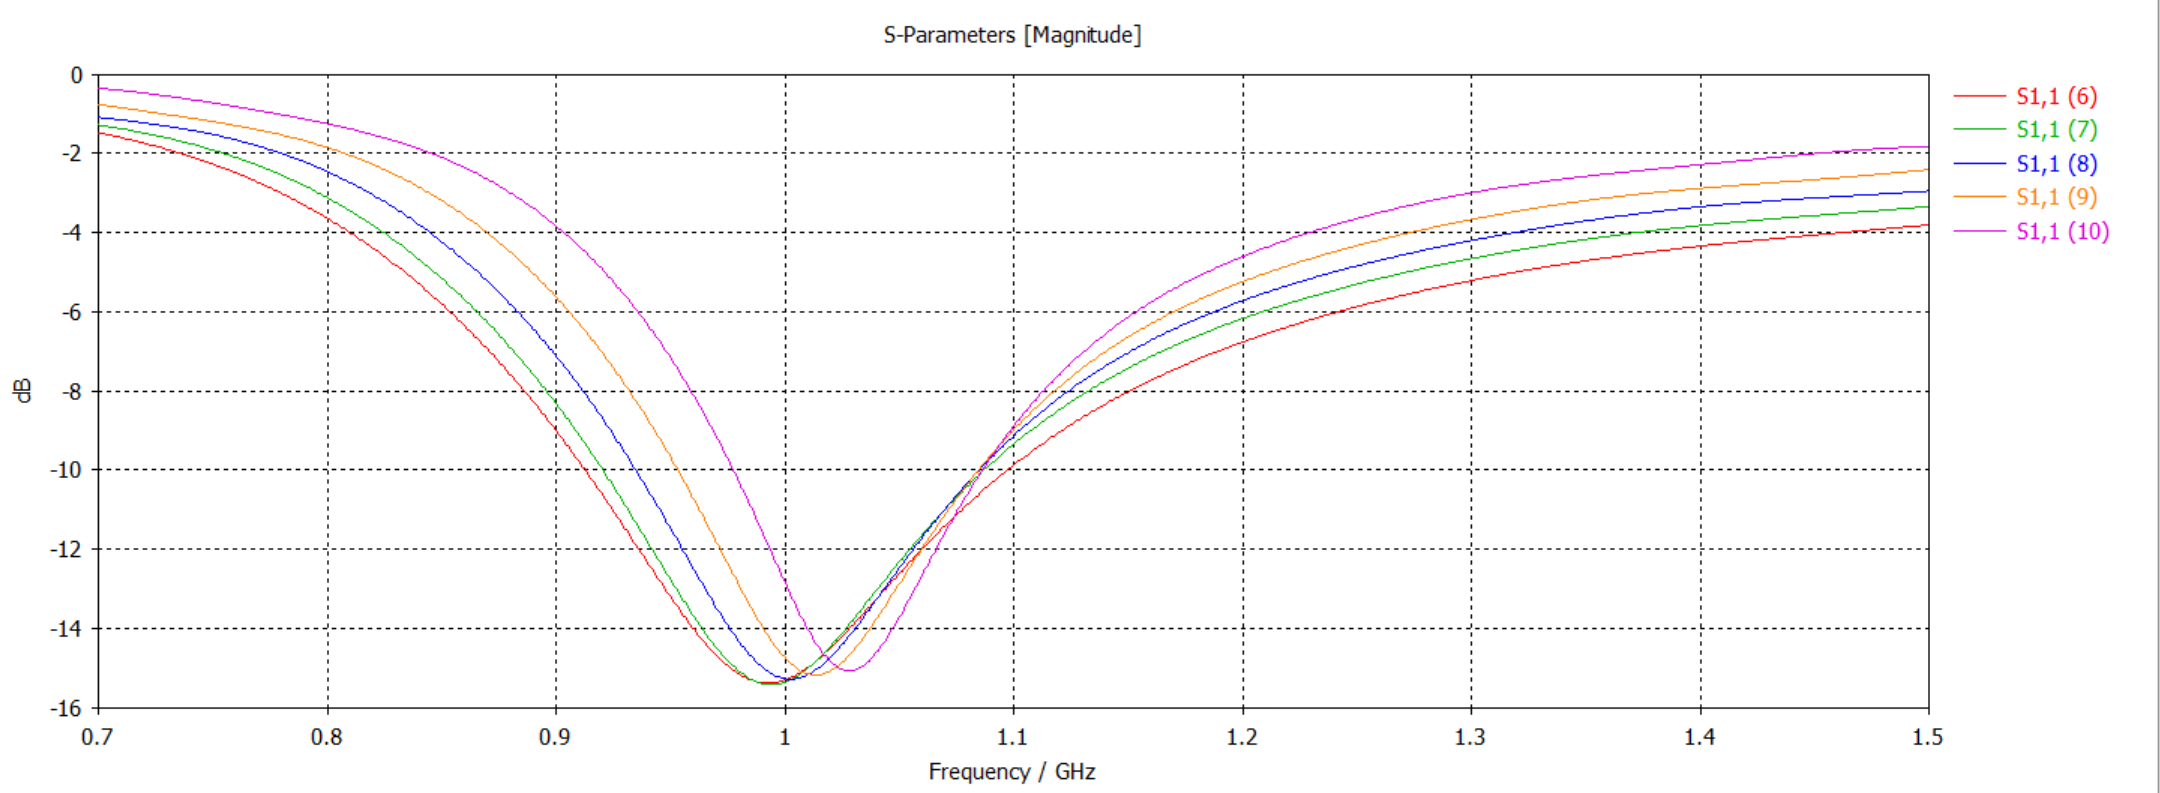
\includegraphics[width=0.8\linewidth]{Lab 1/Data/fractional_bandwidth.png}
    \caption{$|S_{11}|$ from $w = 254 - 50~{\text{mm}}$}
    \label{fig:placeholder}
\end{figure}

\begin{question}What current distribution is observed along the antenna near resonance?
\end{question}
\answer{The surface current following the near-triangular profile we'd expect for an ideal-dipole}
\begin{figure}
    \centering
    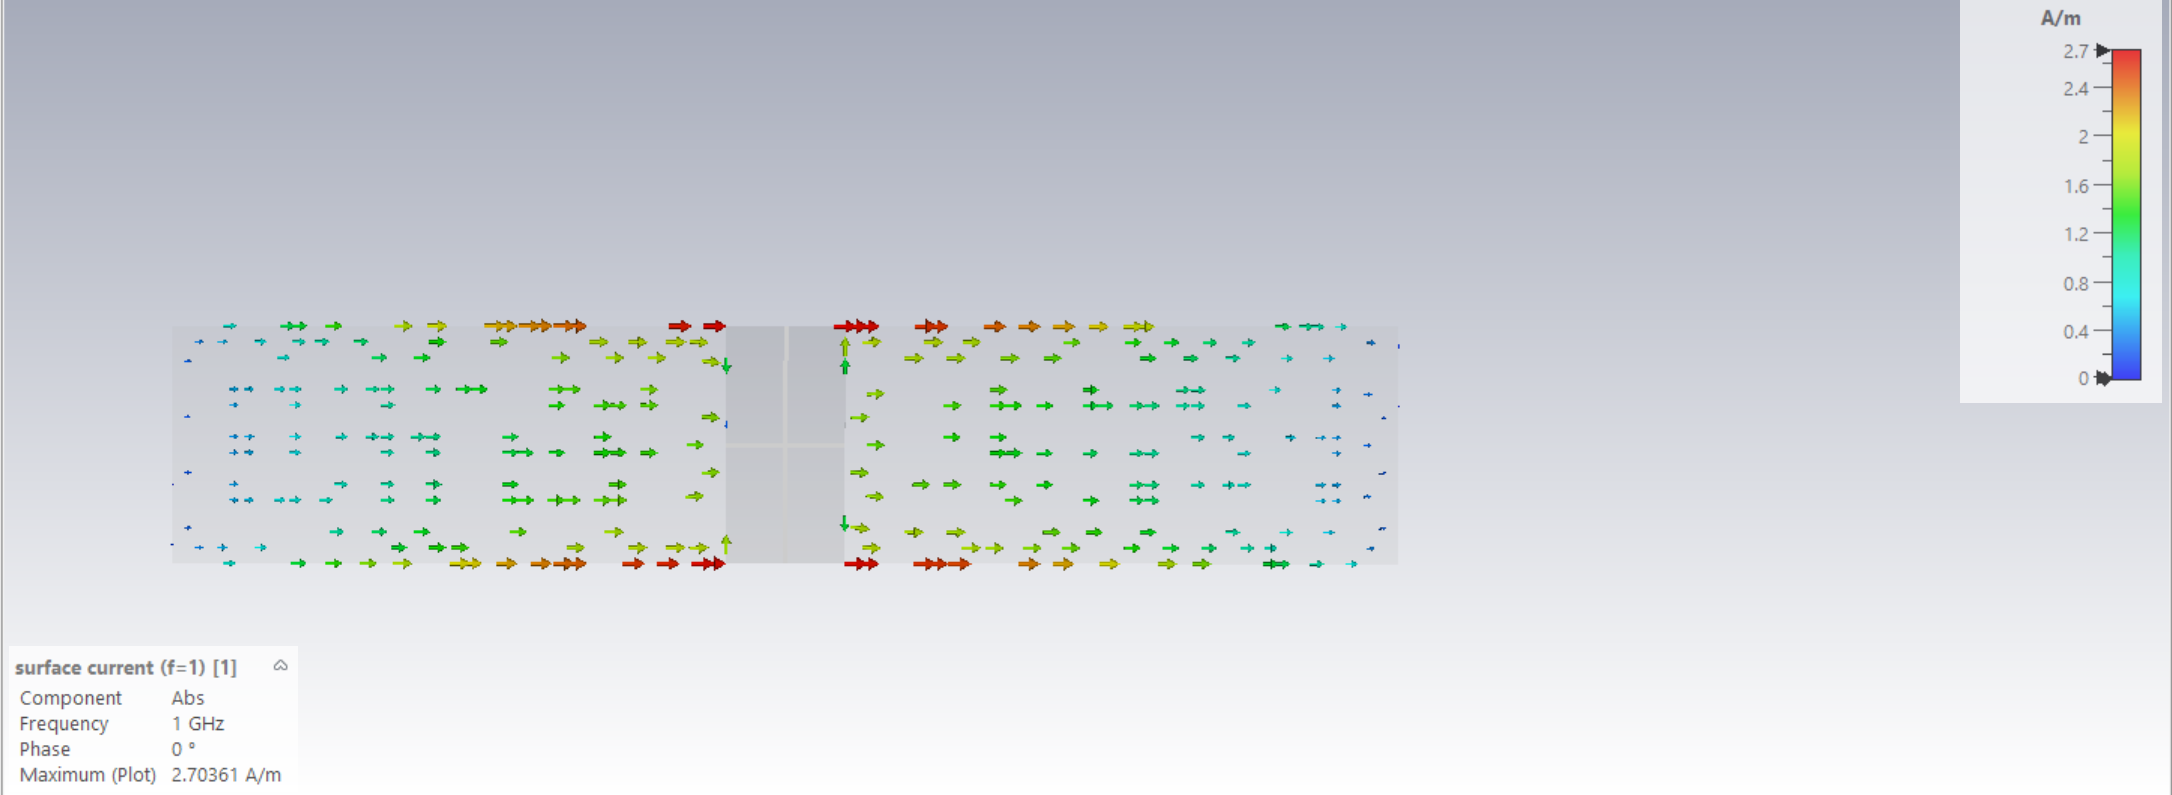
\includegraphics[width=0.8\linewidth]{Lab 1/Data/surface_current.png}
    \caption{Linear Surface Current Plot (2D)}
    \label{fig:placeholder}
\end{figure}

% ═════════════════════════════════════════════════════════════
\section{Fabrication (Exercise 1.3)}

We were not able to procure $1~\text{in}$ copper tape, so our fabricated antenna was modified slightly. We used a foam poster board as a substrate, replacing the $1~\text{in}$ copper tape with $0.5~\text{in}$. The antenna feed was constructed using a SMA to Screw Terminal from Atlas Scientific, with a feed gap matching our simulation design. The following figure shows the antenna after we cut its length down to a quarter wavelength.

\begin{figure}[H]
  \centering
  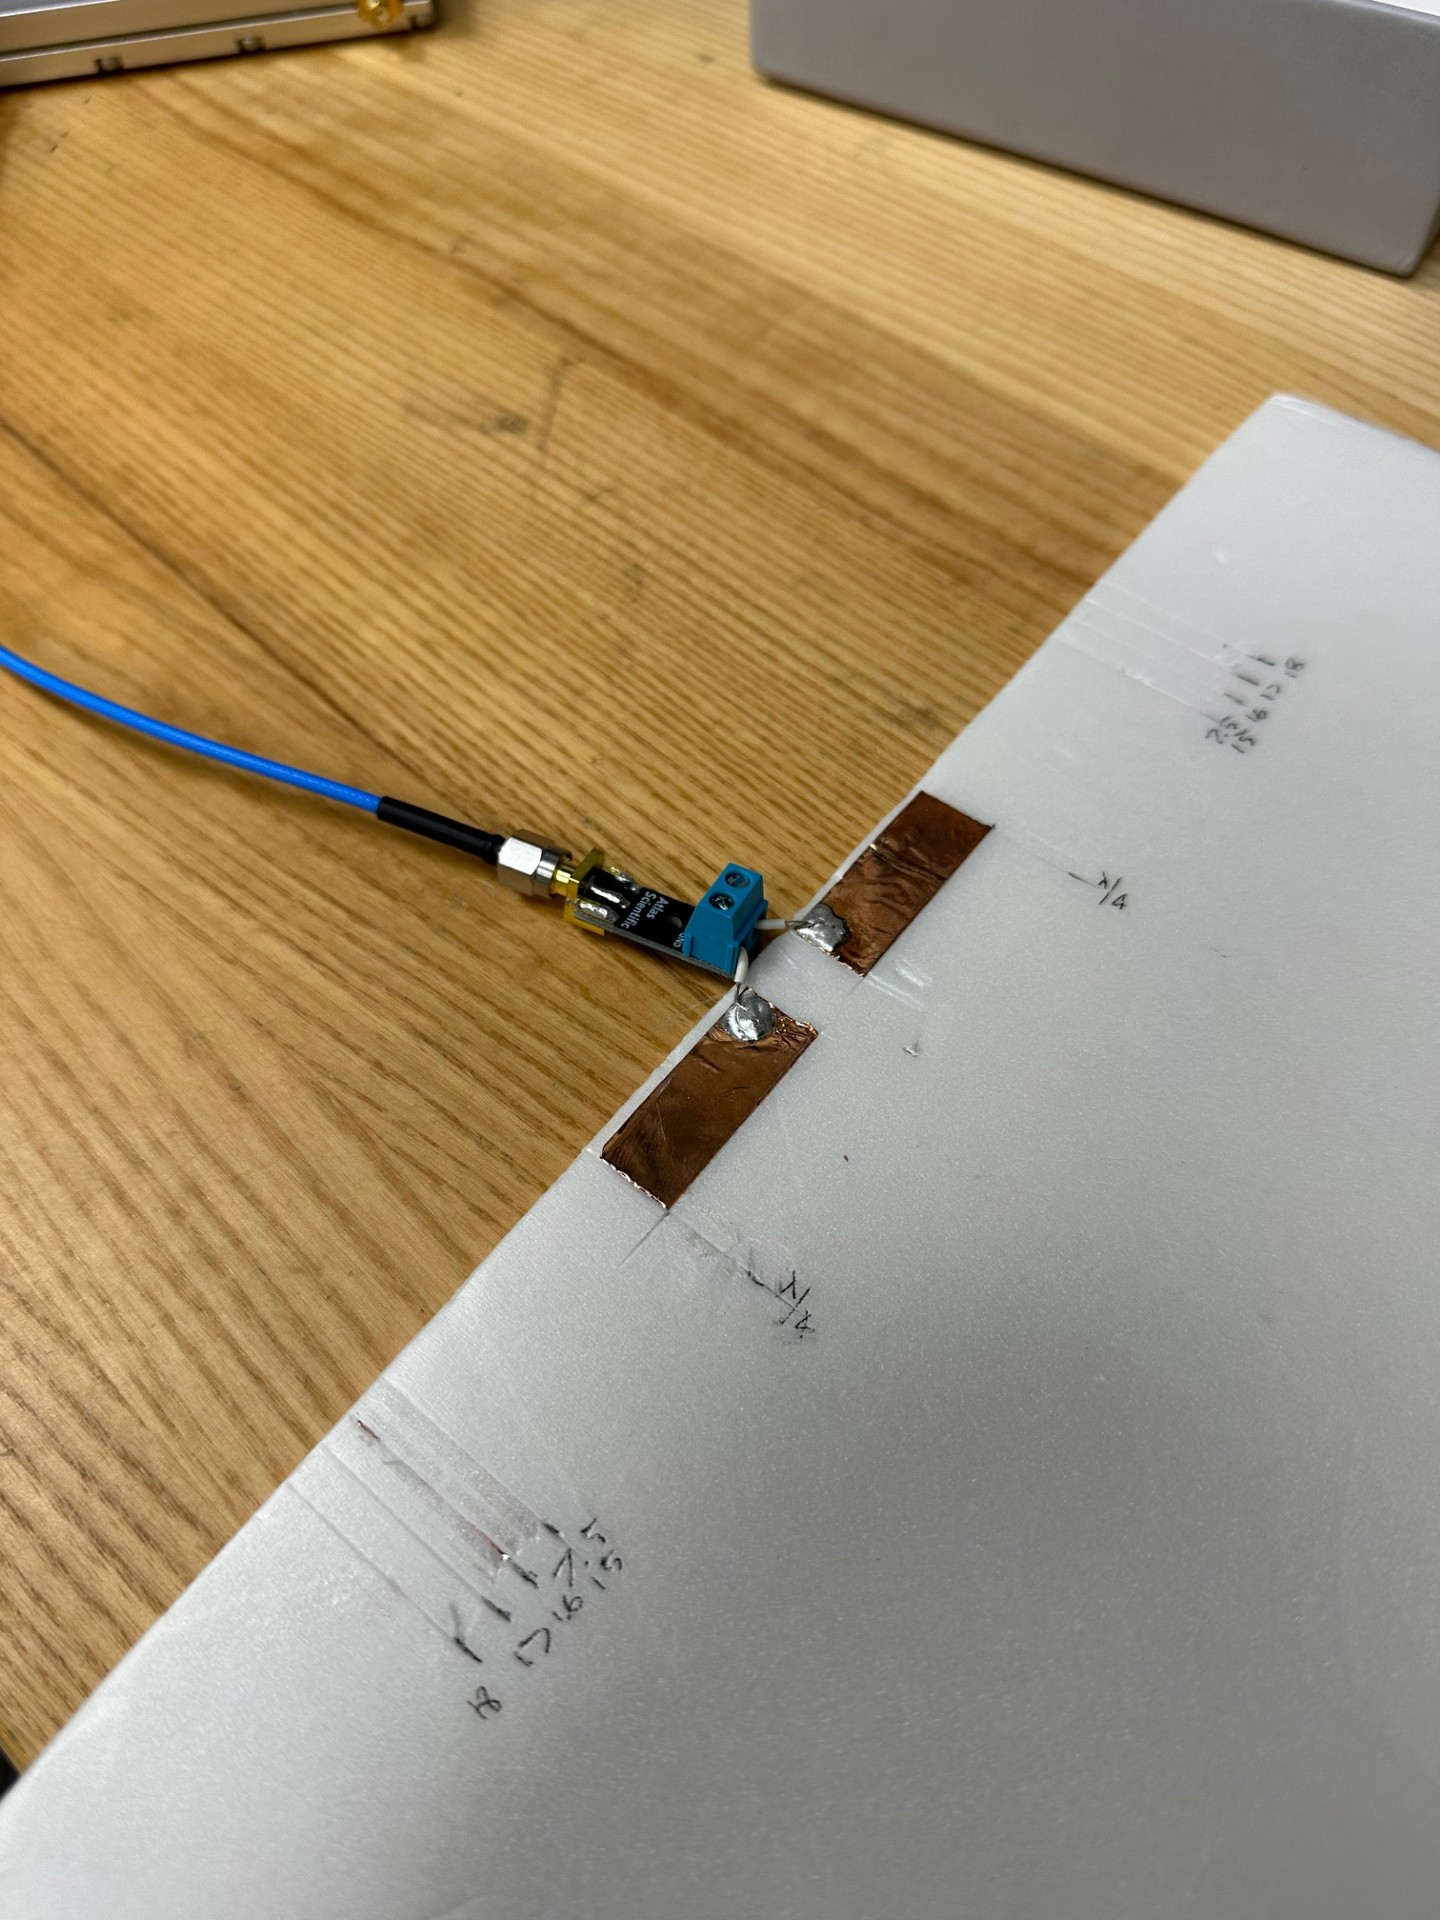
\includegraphics[width=0.5\linewidth]{Lab 1/dipole.jpg}
  \caption{As-built copper-tape dipole.}
  \label{fig:built}
\end{figure}

\begin{table}[H]
  \centering
  \caption{Design vs.\ as-built dimensions.}
  \label{tab:built}
  \begin{tabular}{@{}lcc@{}}
    \toprule
    Dimension & Design & As built \\
    \midrule
    Total length $L$ & \SI{13.1}{mm} & \SIlist{18.5;18;17;16;15}{cm} \\
    Strip width $w$ & \SI{25.4}{mm} & \SI{12.7}{mm} \\
    Feed gap $g$ & \SI{12.7}{mm} & \SI{12.7}{mm} \\
    \bottomrule
  \end{tabular}
\end{table}

% ═════════════════════════════════════════════════════════════
\section{Calibration and Measurement (Exercise 1.4)}

\subsection{Calibration and reference plane}
\todo[LibreVNA SOL calibration over \SIrange{0.5}{1.5}{GHz} (\SI{2}{MHz} steps, 501 points); reference plane at the end of the SMA test cable; adapter and leads not de-embedded (justify). Cable-movement diagnostic result.]

\subsection{Measured $S_{11}$}

\begin{figure}[H]
  \centering
  \includegraphics[width=\linewidth]{\measdir/dipole_s11.png}
  \caption{Measured $|S_{11}|$ of the \SI{1}{in} copper-tape dipole for each length.}
  \label{fig:meas-s11-all}
\end{figure}

\begin{figure}[H]
  \centering
  \begin{subfigure}[b]{0.49\linewidth}
    \includegraphics[width=\linewidth]{\measdir/S11_15.png}
    \caption{Smith chart, $L = \SI{15}{cm}$.}
  \end{subfigure}\hfill
  \begin{subfigure}[b]{0.49\linewidth}
    \includegraphics[width=\linewidth]{\measdir/S11_18.png}
    \caption{Smith chart, $L = \SI{18}{cm}$.}
  \end{subfigure}
  \caption{LibreVNA Smith charts at the shortest and near-resonant lengths. Marker at min $|S_{11}|$.}
  \label{fig:meas-smith}
\end{figure}

% Per-length magnitude/phase screenshots, if wanted (S11_<L>_2.png):
% \includegraphics[width=0.49\linewidth]{\measdir/S11_16_2.png}
% \includegraphics[width=0.49\linewidth]{\measdir/S11_17_2.png}

The input impedance at each marker follows from
\begin{equation}
  Z_\text{in} = 50\,\frac{1 + S_{11}}{1 - S_{11}}~\Omega .
\end{equation}

\begin{table}[H]
  \centering
  \caption{Measured results by length. Minimum $|S_{11}|$ and \SI{-10}{dB} band from the CSV exports; $Z_\text{in}$ from the LibreVNA marker at (or near) the minimum.}
  \label{tab:meas}
  \small
  \begin{tabular}{@{}cccccc@{}}
    \toprule
    $L$ (cm) & $f_{\min|S_{11}|}$ (MHz) & min $|S_{11}|$ (dB) & \SI{-10}{dB} band (MHz) & BW (\%) & $Z_\text{in}$ at marker ($\Omega$) \\
    \midrule
    15   & 1126 & $-12.62$ & 1034--1176 & 12.6 & $72.1 + j19.0$ @ 1128 \\
    16   & 1068 & $-13.14$ & 980--1154  & 16.3 & $70.2 + j17.7$ @ 1088 \\
    17   & 1036 & $-13.95$ & 956--1124  & 16.2 & $72.0 + j12.2$ @ 1038 \\
    18   & 1002 & $-15.53$ & 926--1082  & 15.6 & $68.4 + j6.4$ @ 1002 \\
    18.5 & 996  & $-15.52$ & 902--1070  & 16.9 & $65.5 + j12.0$ @ 1000 \\
    \bottomrule
  \end{tabular}
\end{table}

\noindent\todo[Zero-reactance frequency for each length. The CSVs hold magnitude only, so $X = 0$ cannot be found from them; re-export complex $S_{11}$ (Touchstone \texttt{.s1p}) or read it from the Smith chart.]

% ═════════════════════════════════════════════════════════════
\section{Geometry Study (Exercise 1.5)}

\todo[Resonance shift vs.\ length, measured vs.\ CST. Compare slope $\Delta f / \Delta L$. Optional: quarter-wave (\SI{1}{in} vs.\ \SI{0.5}{in}) result below.]

\begin{figure}[H]
  \centering
  \includegraphics[width=\linewidth]{\measdir/dipole_s11_all.png}
  \caption{All measured cuts including the quarter-wave specimens (\SI{1}{in} and \SI{0.5}{in}) to \SI{6}{GHz}. \todo[Describe the quarter-wave configuration.]}
  \label{fig:meas-qw}
\end{figure}

% Overlay to add once CST is exported (Touchstone/ASCII):
% \begin{figure}[H]
%   \centering
%   \includegraphics[width=\linewidth]{Plots/overlay_s11.png}
%   \caption{Measured vs.\ simulated $|S_{11}|$ for each length.}
%   \label{fig:overlay}
% \end{figure}

% ═════════════════════════════════════════════════════════════
\section{Comparison with Theory (Exercise 1.6)}

\todo[Analytical $R_r$ from the thin-dipole current distribution at each measured length; compare with simulated and measured $R_\text{in}$.]

\begin{table}[H]
  \centering
  \caption{Input resistance: theory, simulation, measurement.}
  \label{tab:compare}
  \begin{tabular}{@{}cccc@{}}
    \toprule
    $L$ (cm) & $R_r$ analytical ($\Omega$) & $R_\text{in}$ CST ($\Omega$) & $R_\text{in}$ measured ($\Omega$) \\
    \midrule
    15   & \todo[...] & \todo[...] & 72.1 \\
    16   & \todo[...] & \todo[...] & 70.2 \\
    17   & \todo[...] & \todo[...] & 72.0 \\
    18   & \todo[...] & \todo[...] & 68.4 \\
    18.5 & \todo[...] & \todo[...] & 65.5 \\
    \bottomrule
  \end{tabular}
\end{table}

\begin{question}How does the analytical radiation resistance compare with the simulated input resistance?\end{question}
\answer{\todo}

\begin{question}How closely does the measured resistance agree with simulation?\end{question}
\answer{\todo}

\begin{question}What physical effects could account for differences?\end{question}
\answer{\todo}

\begin{question}Can the measured input resistance alone establish the antenna's radiation efficiency? Explain.\end{question}
\answer{\todo}

% ═════════════════════════════════════════════════════════════
\section{Discussion}

\subsection*{Resonant length vs.\ half wavelength}
\todo

\subsection*{What determines impedance bandwidth}
\todo

\subsection*{Copper tape vs.\ round wire}
\todo

\subsection*{Feed-cable influence on a balanced antenna}
\todo

\subsection*{VNA accuracy and de-embedding}
\todo

\subsection*{Analytical theory vs.\ numerical simulation}
\todo

% ═════════════════════════════════════════════════════════════
\section{Conclusion}
\todo

\end{document}
